\chapter{Benchmarks}\label{chap:benchmarks}

We created the \tiles library because our port of the \react into the Dart language was slow. 
Natural question arises. Is the \tiles library faster then the \react port into the dart?

\textit{
	We don't compare the \react library with the \tiles library, we compare the port of it into the dart. 
	The main problem in the port performance was the communication between the JavaScript \react library and the implementation created in the Dart language.
}

We measured the time of several distinct scenarios:
\begin{description}
	\item[The mass vs. the structure] \hfill \\
		We will measure the time, needed to render the mass of components in the same level, 
		and to render the complicated structure with lot of branching.
	\item[Creating of the virutal DOM vs. rendering into the real one] \hfill \\
		We measured the time of the construction of the virtual DOM and the render it into the real one. 
		The measurement is compared between the port and the \tiles library.
	\item[Clean vs. dirty updates] \hfill \\
		The last measurement is the comparison of the duration of the updates. 
		We distinguish two types of updates, clean without any change in the virtual DOM and dirty which changes the virtual DOM.
\end{description}

\section{Benchmarking system}\label{sec:benchmarks-system}

We created the benchmarking system, which compares the \react port with the \tiles library.
The system contain the wrapper class, which enable implementation of a common component for both solutions.
We also implements the benchmark component, used for creation of different structures by passing corresponding props.

The benchmark component get props with two important parameters: 
\begin{description}
	\item[levels] is list of numbers, where each number tells, how many children will have the component on each level,
	\item[level] is the level of the current component.
\end{description}

The component render \texttt{levels[level]} children, all with the level bigger by 1.
If the component is at the last level, it renders corresponding number of \texttt{div}s instead of custom components.

By the benchmark component, we are able to test different type of a structure (flat, deep, etc.).

We implemented a runner which obtain run attributes from the hash of the currently opened site. 
The runner enable to run and collect information about benchmarked tasks by running the \textit{content\textunderscore shell} from a command line.

To collect all informations, we created a shell script, which runs the runner with appropriate parameters and output benchmarked times in CSV format.

\section{Mass versus structure}\label{sec:benchmarks-mass-vs-structure}

	From the graph on the \fullref{img:benchmarks-mass-render} we can see, that the \react port is faster 
	in the rendering of the structure composed from one custom component and mass of div components.
	\begin{figure}[h]
	\centering  
		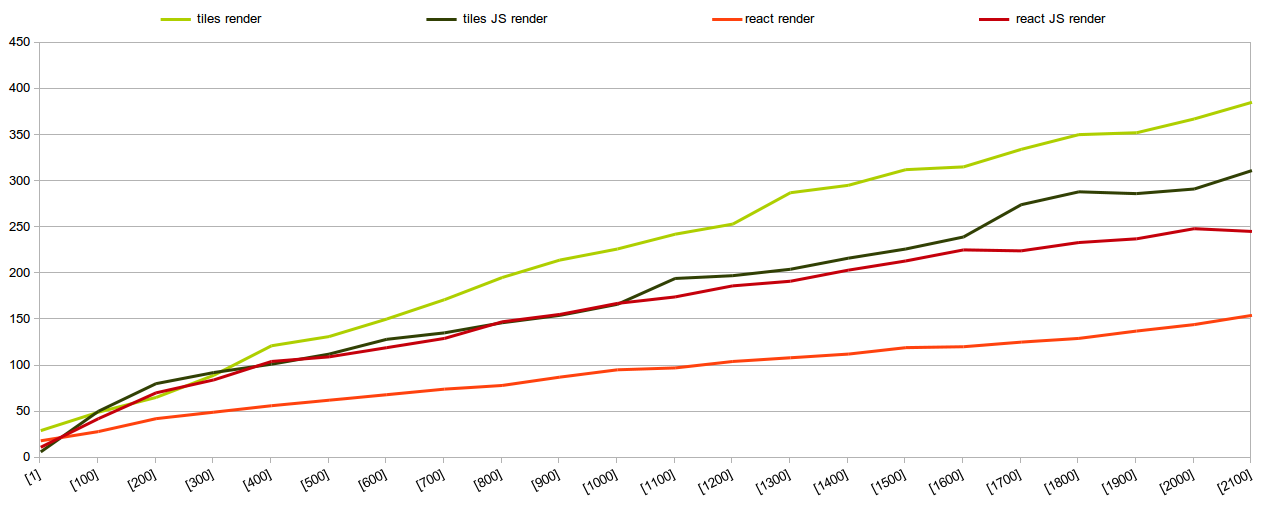
\includegraphics[scale=0.5]{images/benchmarks/m_render.png}
		\caption{Render of simple structure with one custom component and mass of div components}
		\label{img:benchmarks-mass-render}
	\end{figure}

	The graph on the \fullref{img:benchmarks-mass-1-render} shows a big slowdown of the \react port speed with structure 
	of one custom element root with mass of custom elements as children.

	This difference is caused by in Dart implemented life-cycle methods which are called by the JavaScript.
	Where mass of divs don't need to call any custom life cycle methods, the mass of custom component need them. 
	This is also more often scenario, because in the most common case, we want to render the list of some type of data, 
	and for this type of data, we want to create custom reusable component.

	\begin{figure}[h]
	\centering  
		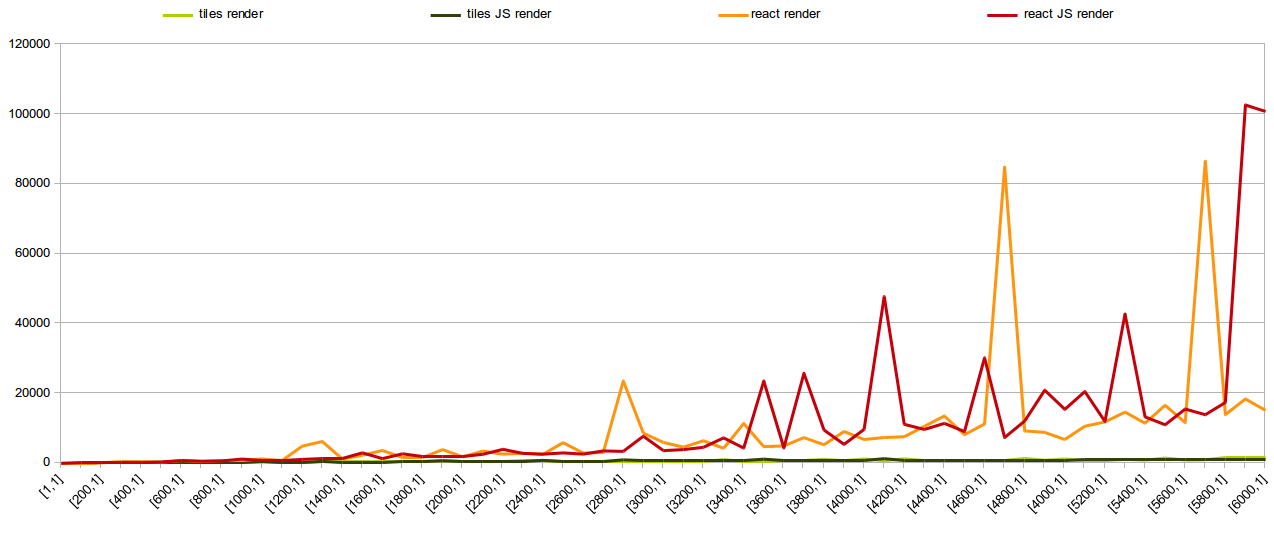
\includegraphics[scale=0.5]{images/benchmarks/m1_render.png}
		\caption{Render of simple structure with one custom component as a root, mass custom component as a child of the root and 1 div components under each of them}
		\label{img:benchmarks-mass-1-render}
	\end{figure}

	On the graph on the \fullref{img:benchmarks-structure-render} we can see the difference between the time of the render of different sizes of the complete binary tree.
	This graph confirm the fact, that for more complicated structures the \react port is slower than the \tiles library.

	\begin{figure}[h]
	\centering  
		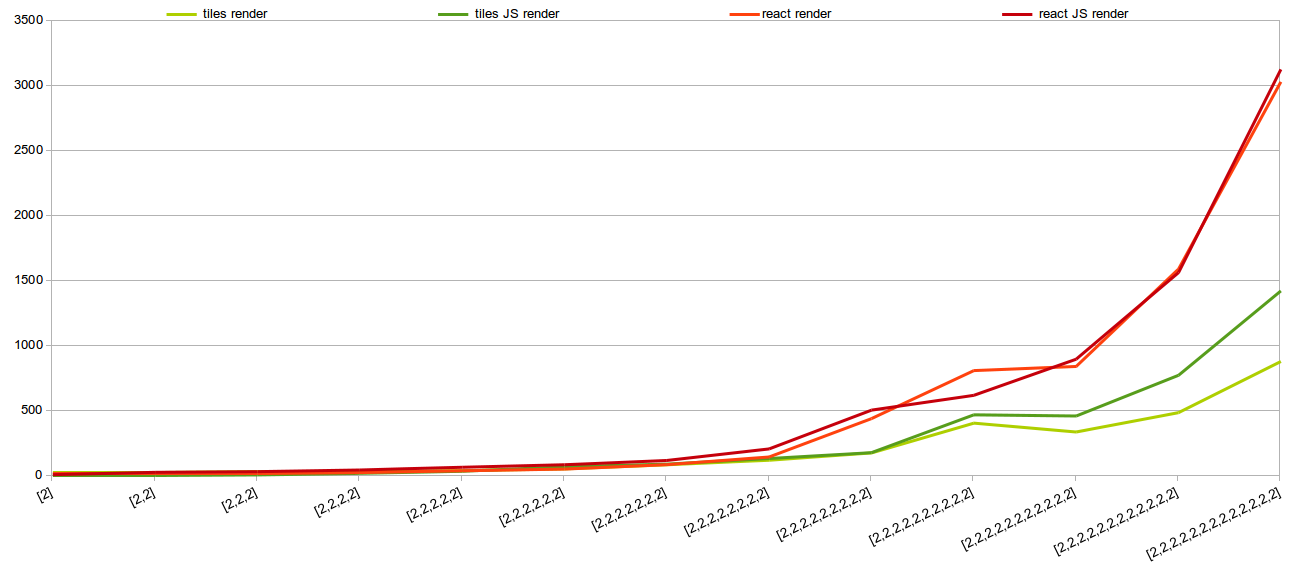
\includegraphics[scale=0.5]{images/benchmarks/s_render.png}
		\caption{Render of the structure of custom components}
		\label{img:benchmarks-structure-render}
	\end{figure}

	The \fullref{img:benchmarks-mass-vs-structure-render} illustrate the fact, that for the flat structures, 
	the \react is constantly faster, but for more complicated structures, the \tiles library perform better.

	\begin{figure}[h]
	\centering  
		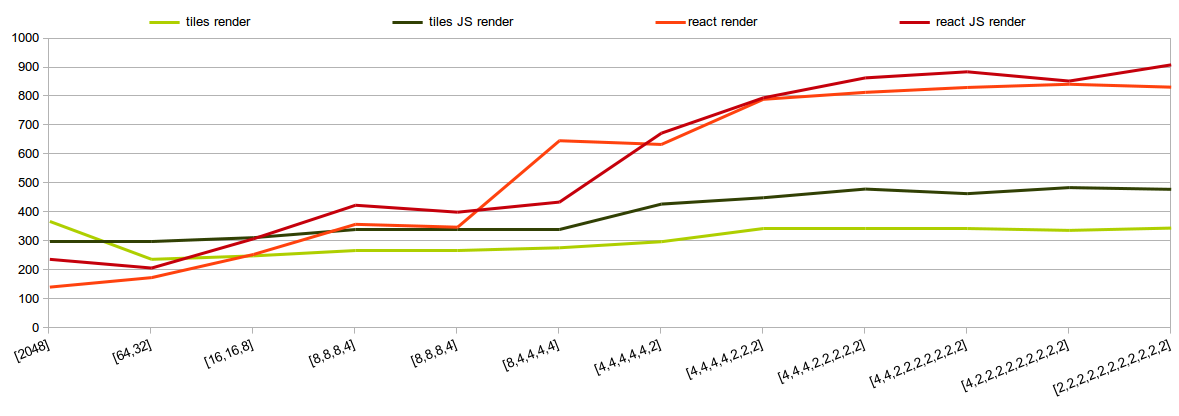
\includegraphics[scale=0.55]{images/benchmarks/mvs_render.png}
		\caption{Comparison of the render of the same number of leafs in the simple, and complicated structure}
		\label{img:benchmarks-mass-vs-structure-render}
	\end{figure}

\section{Clean versus dirty update}\label{sec:benchmarks-clean-vs-dirty-update}

	We compared the clean versus dirty update on the "mass versus structure" results. 
  The performance of the libraries was expected. 
	In bigger structures, where a bigger part of the complete number of components was represented by custom components, 
	the \tiles library was recognizable faster than the \react port.

	\begin{figure}[h]
	\centering  
		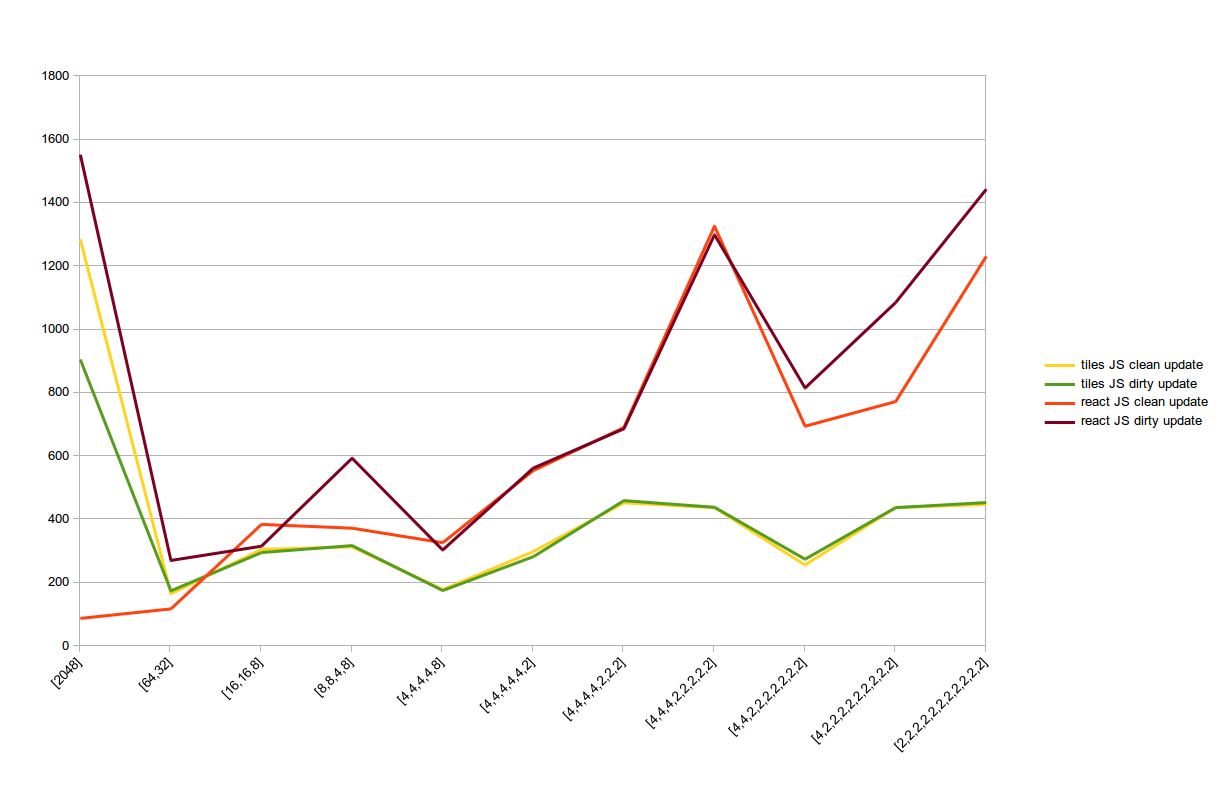
\includegraphics[scale=0.5]{images/benchmarks/mvs_dirty_vs_clean_update.png}
		\caption{Comparison of the clean and dirty update in mass and structure}
		\label{img:benchmarks-mass-vs-structure-dirty-vs-clean-update}
	\end{figure}


\section{Virtual versus real DOM}\label{sec:benchmarks-clean-vs-dirty-update}

	As the most part of the virtual DOM is constructed inside the \texttt{render} method of custom components, 
	we decided to measure the time of the virtual DOM rendering in the \react by measuring the time of the render of all created components.
	We made this decision because we don't have a direct possibility to measure the time of the render of the virtual DOM in the \react port.
	In the \tiles library, we can measure this time directly, as we can build virtual DOM separately.

	On the \fullref{img:benchmarks-mass-vs-structure-virtual-vs-real} we can see that the creation of the virtual DOM is much more optimal in the tiles library, 
	as the \react port need to call Dart functions for all life-cycle methods of the custom component.
	We can also recognize that react can render the existing virtual DOM into the real one more quickly than the \tiles library, 
	but the computation of the virtual DOM is significant in more complicated structures with bigger ratio of custom components.

	\begin{figure}[h]
	\centering  
		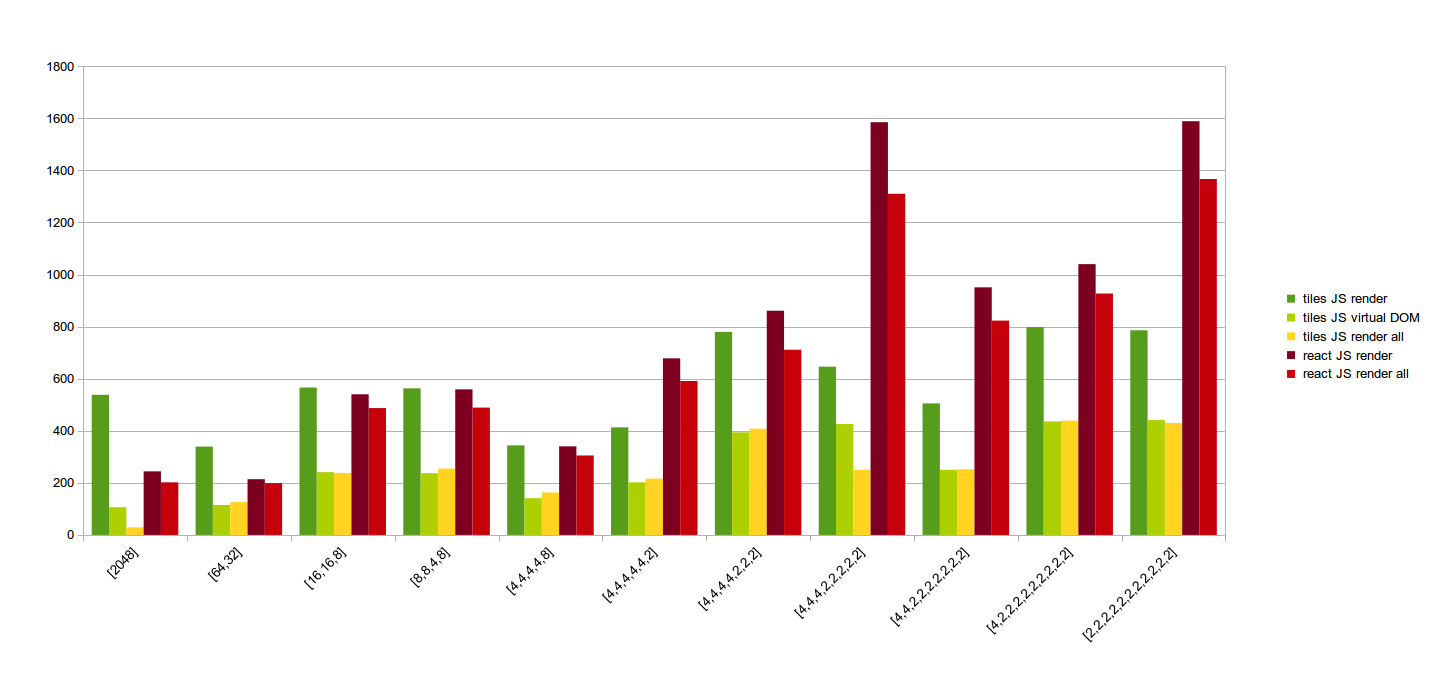
\includegraphics[scale=0.5]{images/benchmarks/mvs_render_vs_virtual_.png}
		\caption{Comparison of the creation of the virtual DOM and rendering into the real DOM in mass and structure}
		\label{img:benchmarks-mass-vs-structure-virtual-vs-real}
	\end{figure}

	In the \fullref{img:benchmarks-structure-virtual-vs-real} is shown the comparison of the render of the virtual DOM and the real DOM of the \react port and the \tiles library in complete binary trees. 
	This comparison also shows that the \tiles library is more efficient than the Dart port of the \react library in thees cases.

	\begin{figure}[h]
	\centering  
		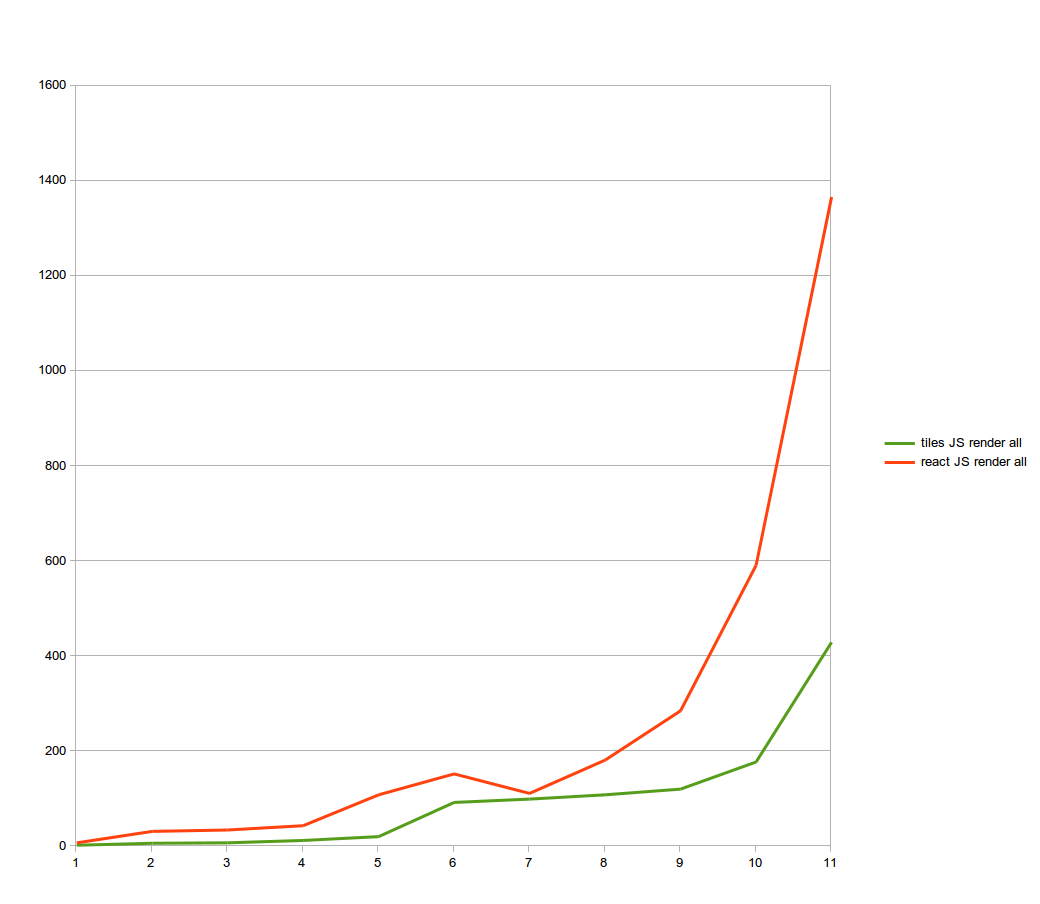
\includegraphics[scale=0.5]{images/benchmarks/s_render_all.png}
		\caption{Comparison of the creation of the virtual DOM and rendering into the real DOM in the structure}
		\label{img:benchmarks-structure-virtual-vs-real}
	\end{figure}

\section{Conclusion}\label{sec:benchmarks-conclusion}

	Benchmarks confirms the theory, that the low performance of the \react port into the Dart language was cause also by the communication between the JavaScript \react library 
	and life cycle methods of custom components implemented in Dart language.
	We further discovered the dependence of the complexity of the virtual DOM structure and the performance ration of the \tiles library and the \react port.
	This dependence was partly caused by bigger ration of custom components.

	\textit{At the end of the Benchmarks chapter we want to acknowledge once more, that we didn't compare the \react and the \tiles library, but the Dart port of the \react library with the \tiles library.
	The biggest problem of the Dart port of the \react library was the communication between the Dart and the JavaScript.}
